\section{Consideraciones}
Se decidi'o dejar los aspectos asincr'onicos del juego del truco fuera del alcance del trabajo, ya que el foco est'a en la parte criptogr'afica del mismo.
Por lo tanto, se implement'o una simplificaci'on del juego en la cual los turnos de juego est'an bien definidos, y cada jugador debe esperar su turno para poder jugar una carta o realizar alg'un canto. Esta simplificaci'on no trae grandes inconvenientes a la hora de jugar, pero simplifica notablemente la implementaci'on del juego, ya que permite prescindir del uso de threads, evitando cualquier posible condici'on de carrera (por ejemplo si un jugador canta \"truco\" pero el otro tambi�n cantra "truco" antes de recibir el canto del primero).
De esta manera, el jugador que debe bajar una carta es el que tiene el turno. Si en lugar de jugar una carta, decide hacer un canto, cede su turno moment'aneamente y s'olo hasta que el contrincante conteste el canto. Una vez realizados los intercambios de turno requeridos por el canto realizado, el turno vuelve al jugador que deb'ia bajar una carta.

Se decidi'o dividir el sistema en distintos m'odulos, cada uno con su responsabilidad bien definida. Toda la l'ogica necesaria para poder jugar al Truco y manejar los turnos se encuentra en el m'odulo ManoTruco. El m'odulo red se encarga de mantener una conexi'on TCP entre los jugadores, mientras que el m'odulo L'ogica de red es el que implementa el protocolo dise'nado, utilizando los m'odulos RSA y AES seg'un corresponda, y brindando una interfaz que permita al resto del sistema enviar y recibir jugadas de cartas y cantos. El m'odulo main es el que implementa la interfaz con el usuario, y usando una instancia de ManoTruco y una de Logica de red se encarga coordinar y llevar adelante la mano de truco.
En el siguiente diagrama se muestran los m'odulos mencionados y c'omo se relacionan entre s'i.

\begin{figure}
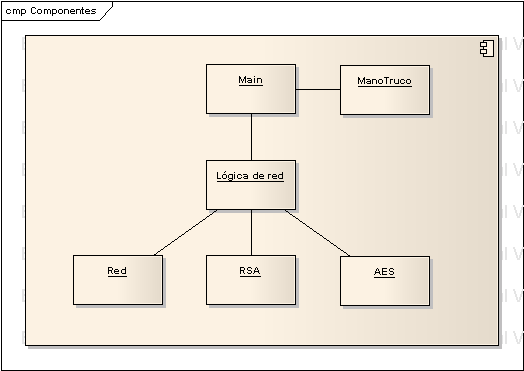
\includegraphics{Componentes.png}
\end{graphics}
